\subsection{Monitoraggio e Intervento}
L'utilizzo della suite \textbf{Ipopt} e' stato fatto per l'applicazione di un sistema
di monitoraggio e intervento all'interno del modello di simulazione. Successivamente l'idea
di utilizzare un integrazione con la suite \textbf{SciML.ai} verra' sfruttata per 
aggiungere algoritmi di Machine Learning per rendere piu' realistico e consistente il modello 
nelle sue predizioni e scelte.

\subsubsection{Controllore con Ipopt}

\begin{minipage}{\linewidth}
	\centering
	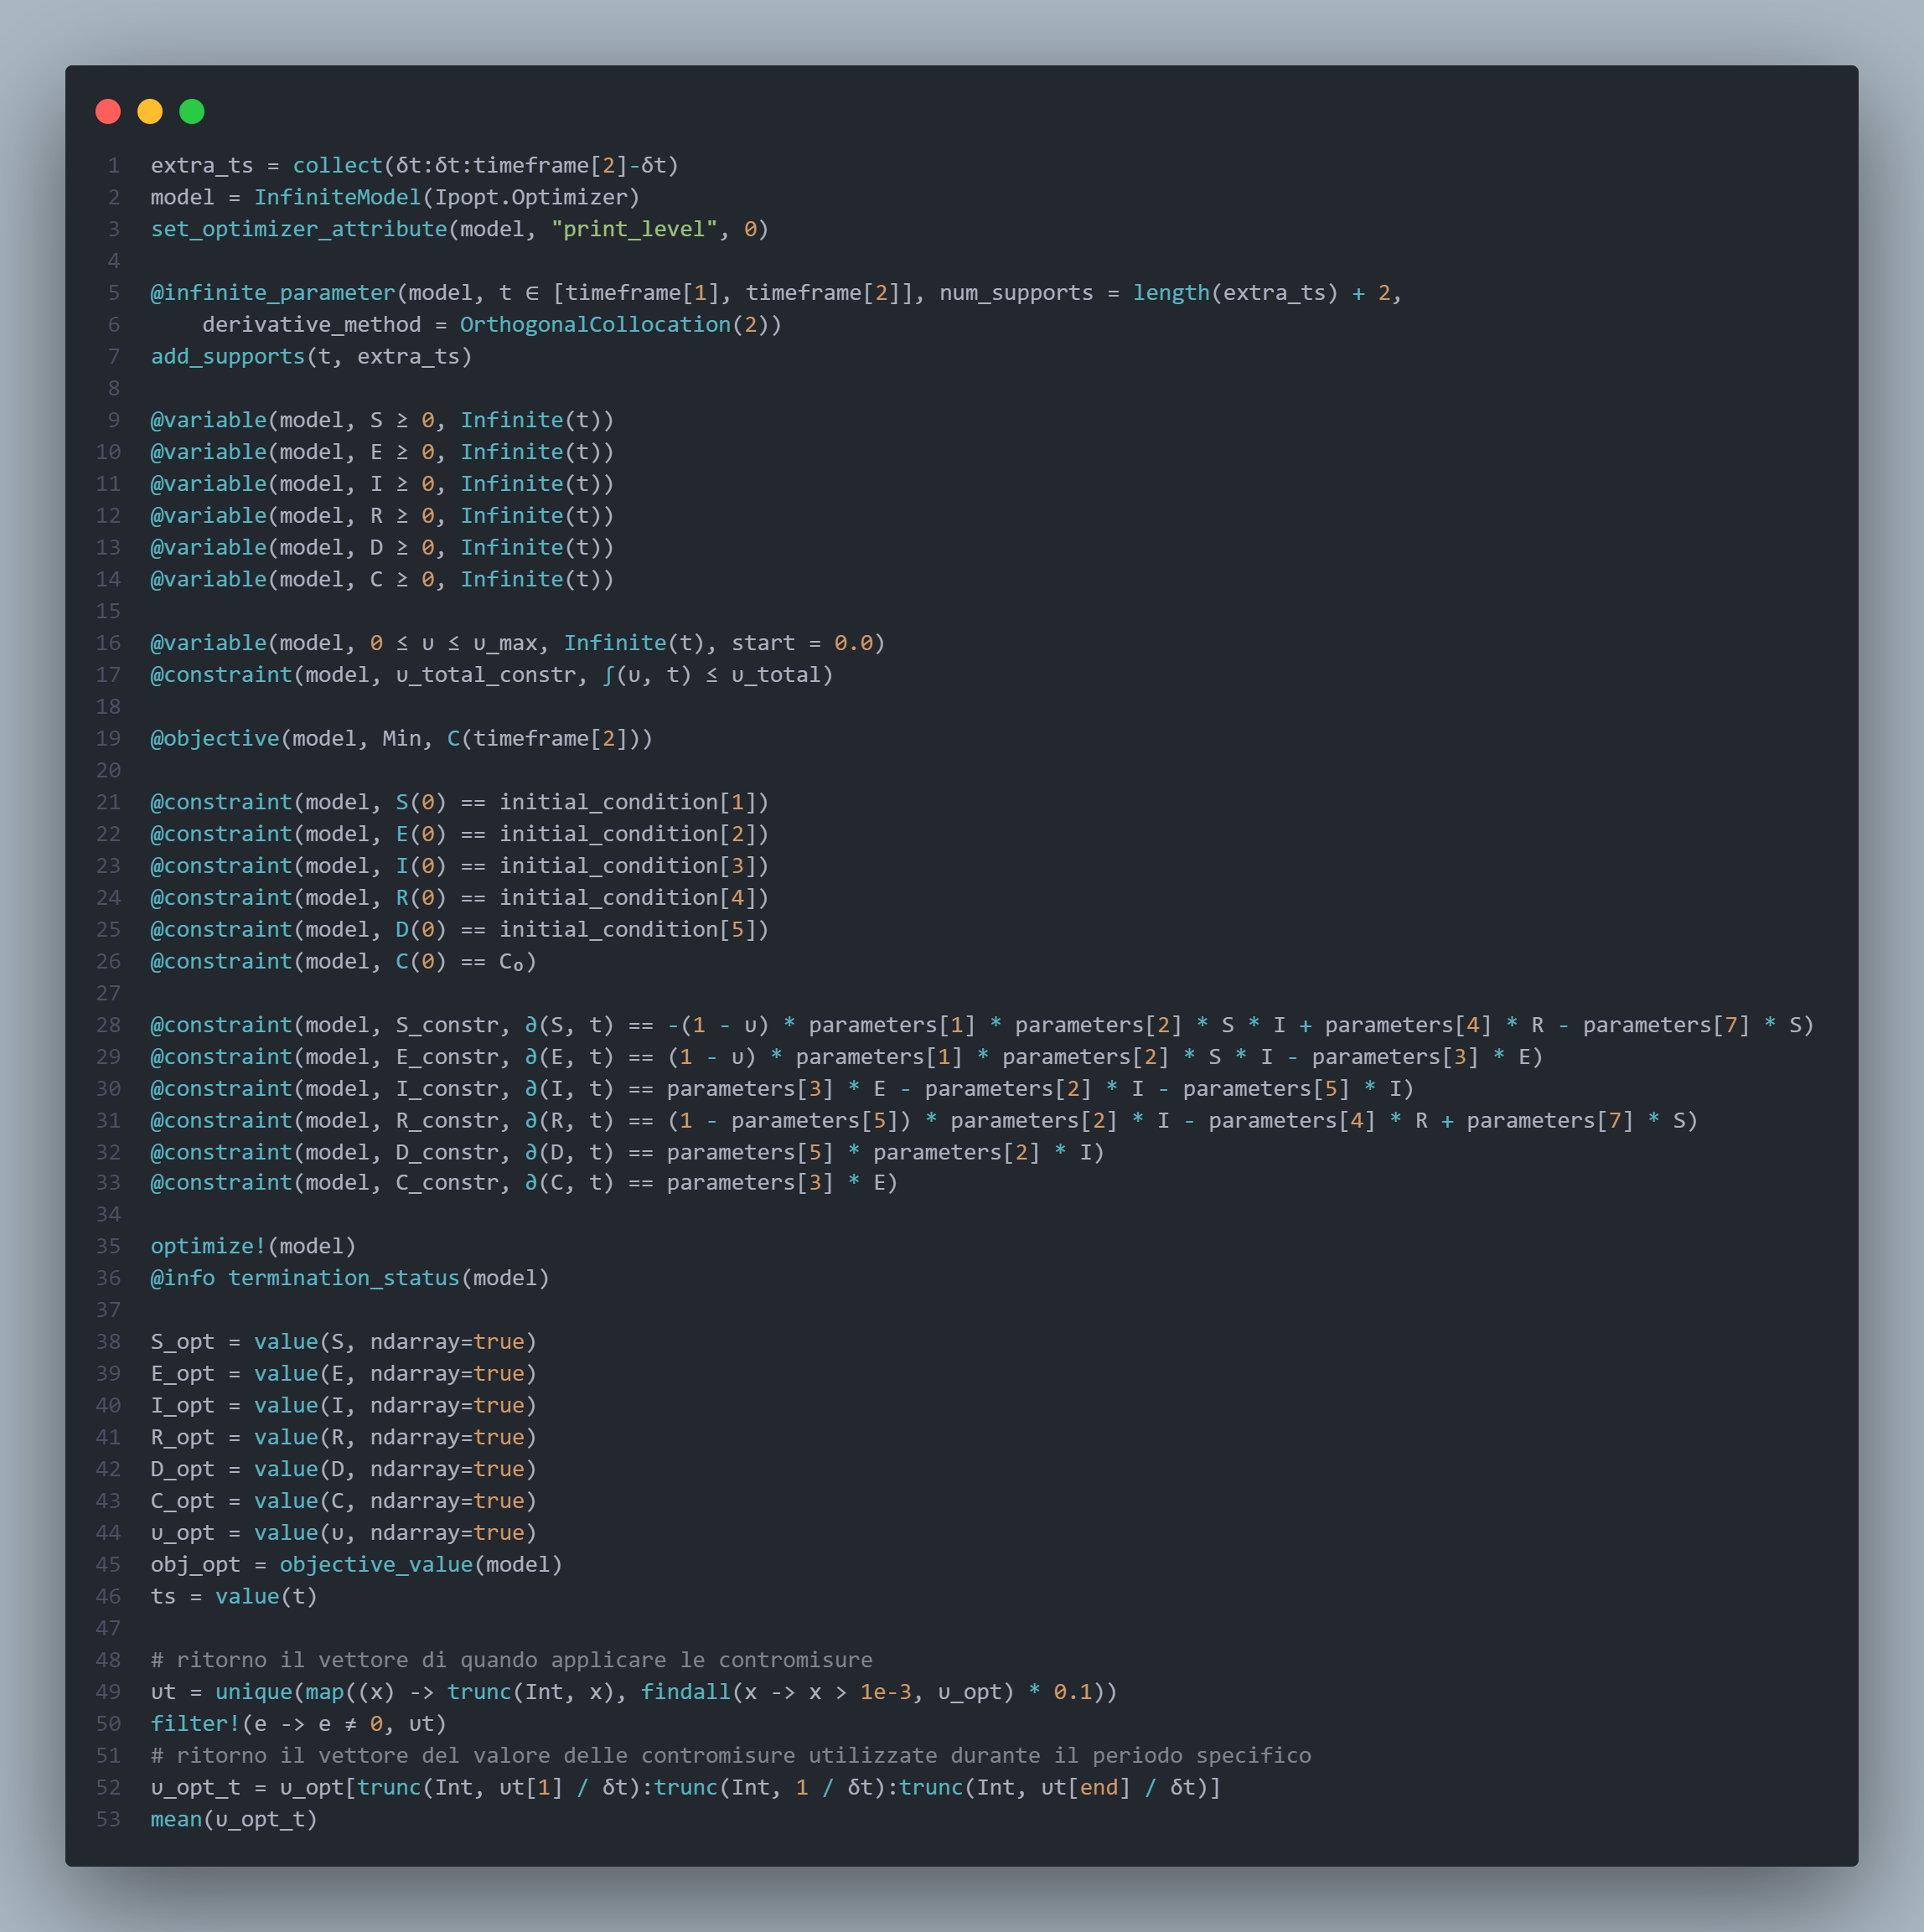
\includegraphics[width=\textwidth]{img/controller_ipopt.png}
	\captionof{figure}{Definizione del controllore tramite Ipopt}
	\label{fig:controller_ipopt}
\end{minipage}

L'approccio generale e' stato semplice ma efficace, in quanto viene definito un modello 
per raccogliere tutte le informazioni relative e necessarie per l'algoritmo di ottimizzazione
e successivamente vengono definite le regole che governano il comportamento del modello. 

Le regole in questione sono principalmente le stesse che sono usate per descrivere il modello SEIR
che viene utilizzato all'interno del modello ad agente.

\begin{minipage}{\linewidth}
	\centering
	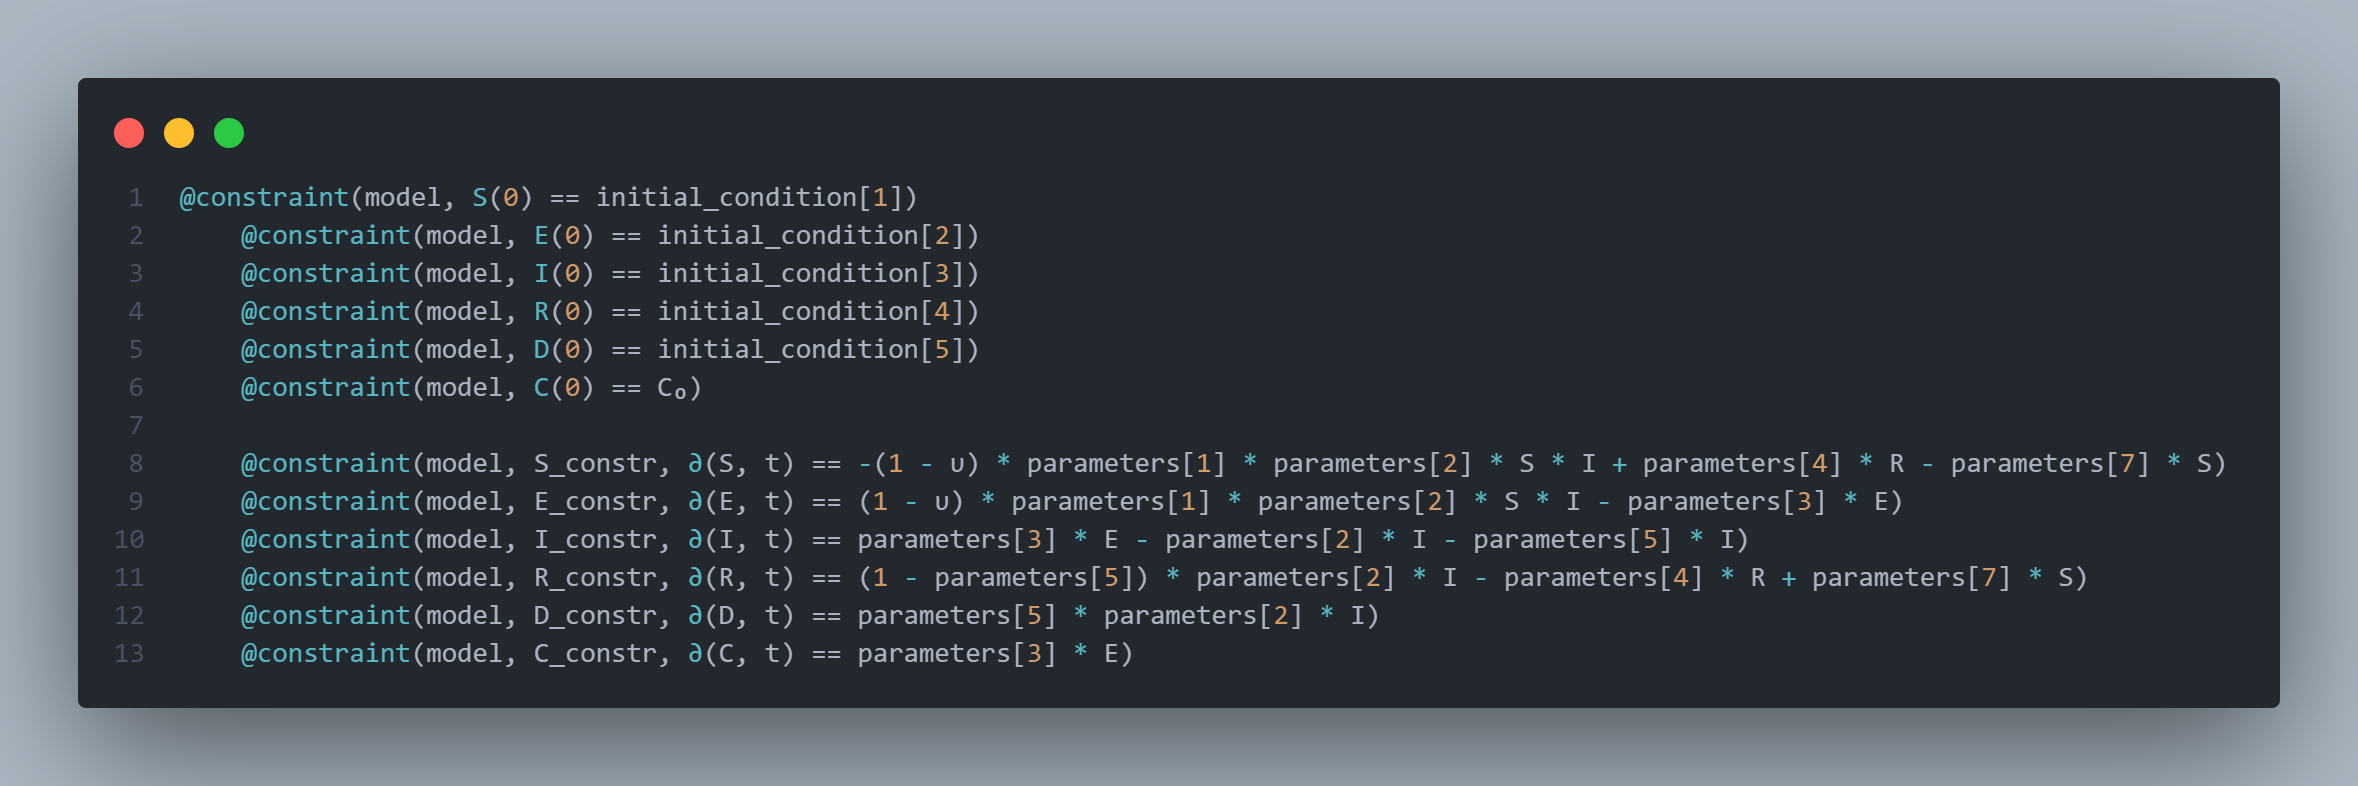
\includegraphics[width=\textwidth]{img/controller_rules.png}
	\captionof{figure}{Definizione regole del modello del controller}
	\label{fig:controller_rules}
\end{minipage}

Essendo che le regole mostrate in figura \ref{fig:controller_rules} sono relative agli stati 
SEIR e l'idea alla base del controllore e' quella di ridurre quanto piu' possibile il numero di
infetti cumulati che ci sono all'interno del sistema, e' stato aggiunto uno stato che descrive
appunto questo stato aggiuntivo.

Successivamente vi sono delle regole su quanto il modello puo' impiegare in termini di risorse, 
le quali sono le nostre contromisure con relativo costo, dato dall'integrale del valore della nostra
contromisura applicata nel tempo.

\begin{minipage}{\linewidth}
	\centering
	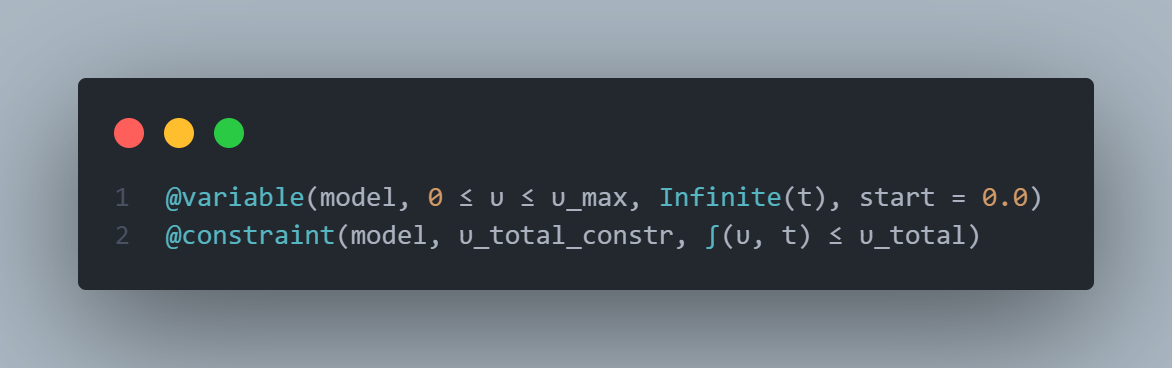
\includegraphics[width=\textwidth]{img/controller_rules_1.png}
	\captionof{figure}{Definizione regole del modello del controller per le contromisure}
	\label{fig:controller_rules_1}
\end{minipage}

Infine viene ottimizzato il modello e ritornato il valore medio delle contromisure applicate
quando applicate. 

\subsubsection{SciML.ai}

L'utilizzo della suite \textbf{SciML.ai} e' stato fatto per l'integrazione
di un modello di Machine Learning in un sistema di monitoraggio e possibilmente di 
intervento. Applicare un algoritmo di ML per predire l'andamento di un sistema non lineare dinamico 
senza avere una grande base di dati puo' risultare problematico e i risultati possono risultare 
poco affidabili. Lo sviluppo di tecniche che congiungono la modellazione puramente matematica
alla flessibilita' delle reti neurali ha permesso di sviluppare approcci \emph{data-driven domain-specific} 
\cite{rackauckas2020universal} \cite{Kim_2021} \cite{dandekar2022bayesian} \cite{chen2019neural}
che permettono di ottenere risultati affidabili pur avendo una base di dati scarsa.

\subsubsection*{Addestramento}
Viene definito il sistema di ODE che fara' da base per l'addestramento della \textbf{Neural ODE} \cite{chen2019neural}
e successivamente viene definita la rete neurale tramite la suite \textbf{Lux.jl} \cite{pal2023lux}.
Questo permette di definire facilmente e velocemente una rete neurale che verra' usata 
in coppia con il sistema di ODE per ottenere il meglio da entrambi, andando a definire 
quello che viene chiamato \textbf{Scientific Machine Learning}.

\begin{figure}[!hb]
	\centering
	\begin{subfigure}[b]{0.45\textwidth}
		\centering
		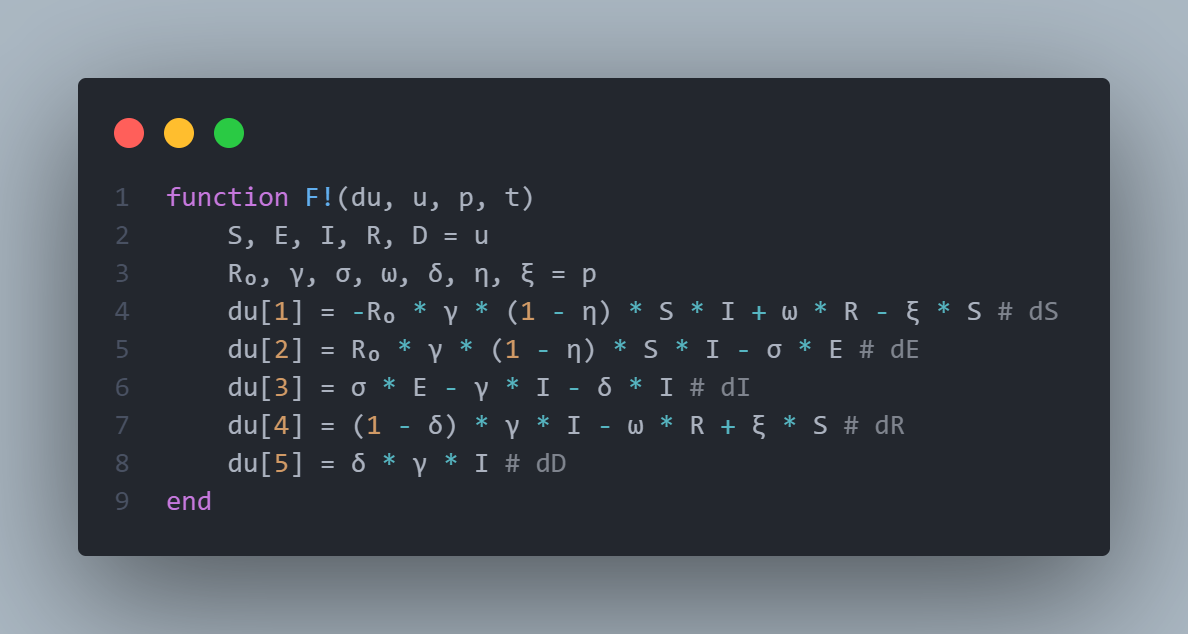
\includegraphics[width=\textwidth]{img/seir_function.png}
		\caption{Definizione del sistema di ODE per l'addestramento della rete neurale}
		\label{fig:seir_function}
	\end{subfigure}
	\hfill
	\begin{subfigure}[b]{0.45\textwidth}
		\centering
		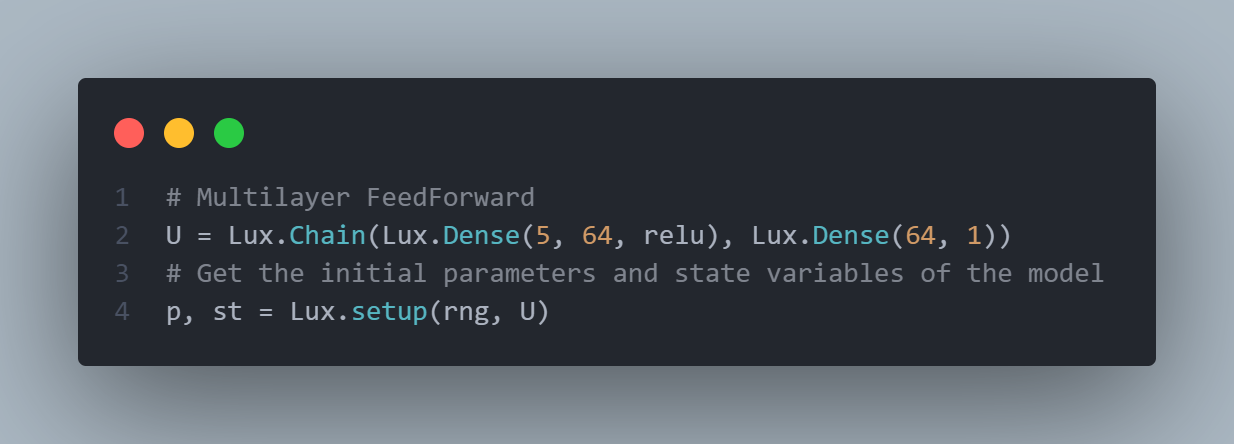
\includegraphics[width=\textwidth]{img/neural_ode.png}
		\caption{Definizione della rete neurale}
		\label{fig:neural_ode}
	\end{subfigure}
\end{figure}

Dopo aver definito queste due funzioni, vengono definite le regole di predizione
per l'addestramento e le regole della funzione di loss. La funzione di loss viene definita 
come la loss L2 ovvero un \textbf{Mean Squared Error (MSE)} o \textbf{Errore Quadratico Medio}
\cite{wiki:Mean_squared_error}.

\begin{figure}[!hb]
	\centering
	\begin{subfigure}[b]{0.45\textwidth}
		\centering
		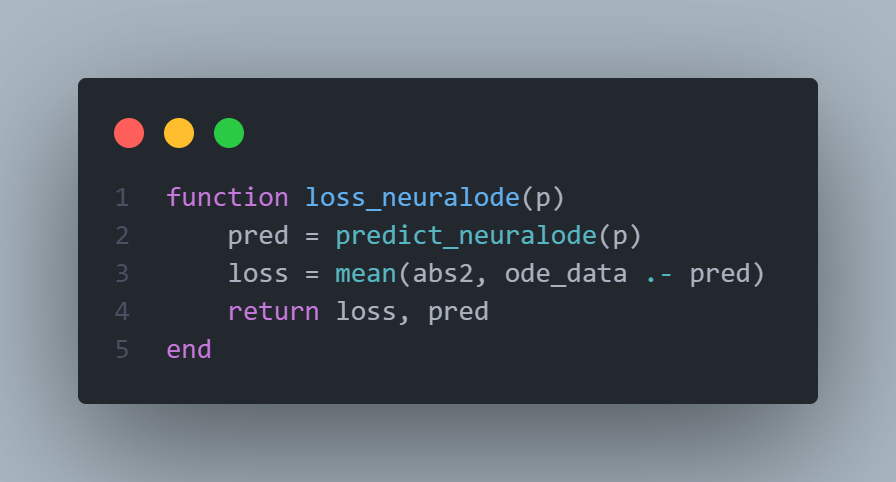
\includegraphics[width=\textwidth]{img/loss.png}
		\caption{figure}{Definizione della funzione di Loss}
		\label{fig:loss_function}
	\end{subfigure}
	\hfill
	\begin{subfigure}[b]{0.45\textwidth}
		\centering
		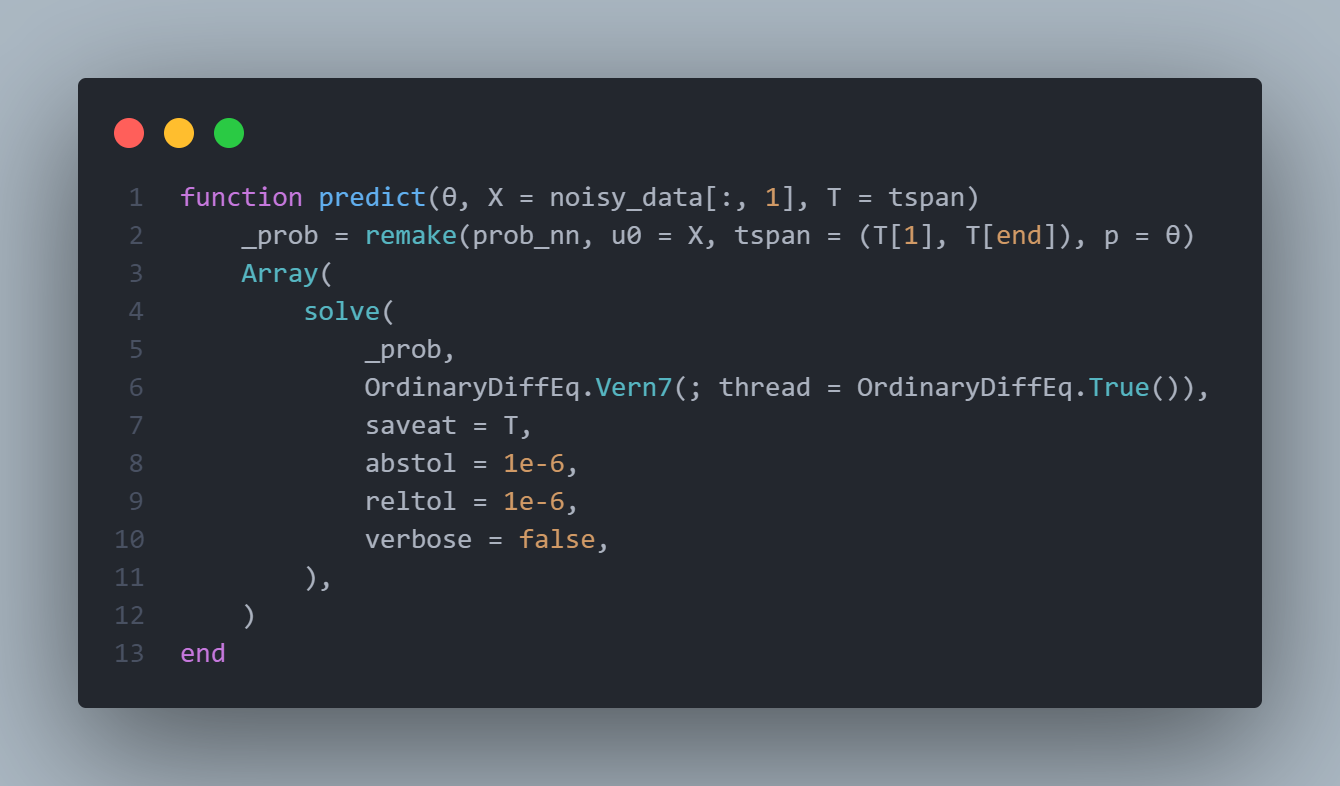
\includegraphics[width=\textwidth]{img/predict_function.png}
		\caption{Definizione del loop di addestramento}
		\label{fig:predict_function}
	\end{subfigure}
\end{figure}

Utilizzando poi le regole di ottimizzazione offerte dal framework \textbf{Optimization.jl} \cite{vaibhav_kumar_dixit_2023_7738525}
e' possibile definire una struttura di controllo tramite la creazione di un 
\textbf{OptimizationProblem} e una \textbf{OptimizationFunction} e la scelta di un 
algoritmo di ottimizzazione, generalmente lasciato automatico, e' possibile addestrare
la propria \emph{Neural ODE}.

\begin{minipage}{\linewidth}
	\centering
	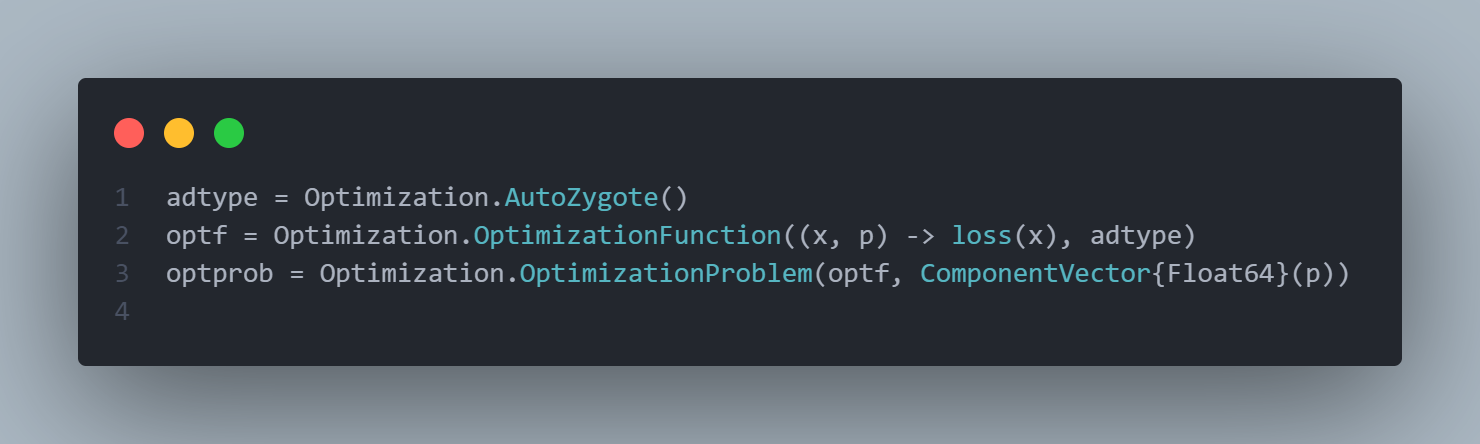
\includegraphics[width=\textwidth]{img/optimization_functions.png}
	\captionof{figure}{Definizione delle funzioni di ottimizzazione}
	\label{fig:optimization_function}
\end{minipage}

Per ottenere il massimo dall'addestramento vengono effettuati due cicli di addestramento, 
uno usando un determinato ottimizzatore, \textbf{ADAM} e successivamente utilizzando quel 
risultato, fare un altro ciclo di addestramento con un ottimizzatore differente, in questo 
caso \textbf{BFGS} \cite{10.1093/imamat/6.1.76} \cite{10.1093/comjnl/13.3.317} 
\cite{35d0019d-775a-3628-b0b4-67be112e346b} \cite{e3177091-3094-3792-9d61-0ab445735ddb}.

Questo procedimento viene effettuato principalmente perche' si cerca di sfruttare al meglio le
proprieta' dei vari ottimizzatori. In primo luogo si utilizza ADAM per la maggior parte delle 
iterazioni, andando a sfruttare e massimizzare la sua capacita' di trovare una buona area 
generale dello spazio dei parametri. Successivamente per una manciata di iterazioni viene utilizzato 
BFGS che velocemente riesce a cadere in un buon minimo locale. 

Se si utilizzasse solamente ADAM si andrebbe probabilmente incontro ad una richiesta in 
termini di iterazioni molto alta, rispetto al risultato complessivo, e viceversa
se si utilizzasse solo BFGS si andrebbe incontro ad un brutto minimo locale.

\begin{minipage}{\linewidth}
	\centering
	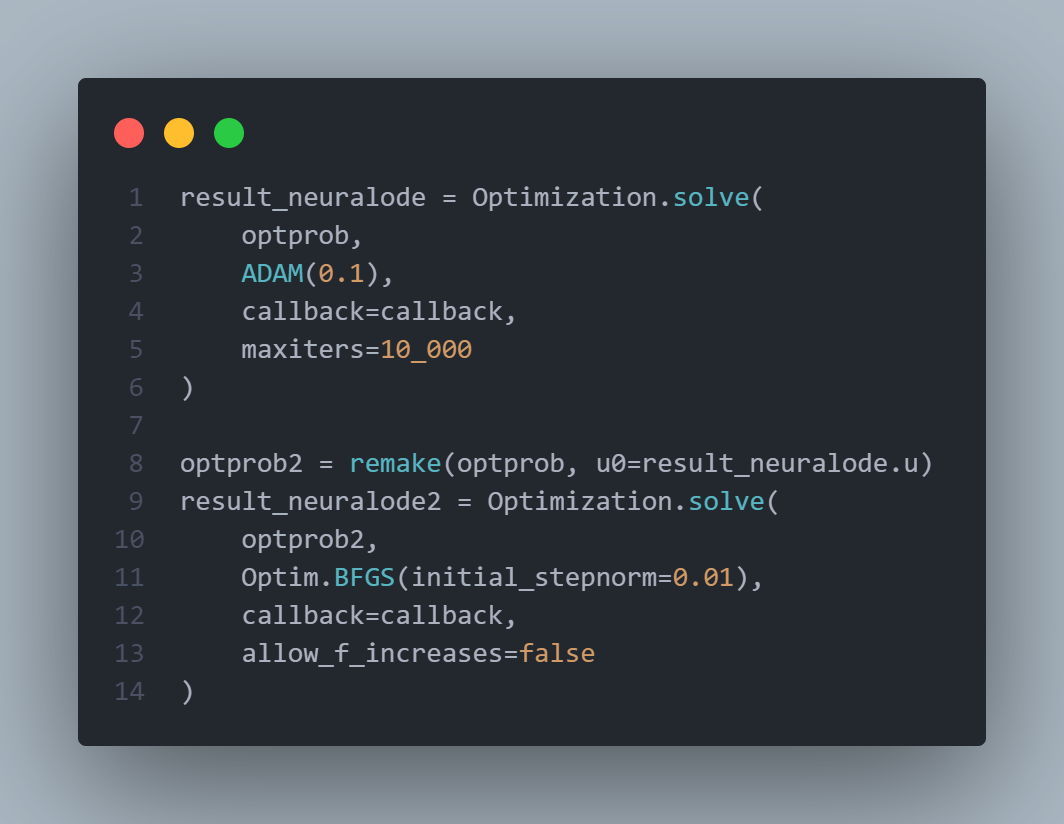
\includegraphics[width=\textwidth]{img/training.png}
	\captionof{figure}{Definizione delle funzioni di addestramento tramite due differenti ottimizzatori}
	\label{fig:training_function}
\end{minipage}

\subsubsection*{Predizione}
Viene utilizzato un approccio simile a quello denominato SINDy \cite{wiki:Sparse_identification_of_non-linear_dynamics}
per effettuare predizioni sul lungo termine fondendo un approccio \textbf{DataDriven} ad uno
\textbf{Domain Specific}.  

DESCRIZIONE DI COS'E' SINDy E IMMAGINI VARIE

\subsubsection{Grafici}